% !TEX root = main.tex
%%%%%%%%%%%%%%%%%%%%%%%%%%%%%%%%%%%%%%%%%%%%%%%%%%%%%%%%%%%%%%%%%%%%%%%%%%%%%%%%
% Viewing and Cleaning the Data
%%%%%%%%%%%%%%%%%%%%%%%%%%%%%%%%%%%%%%%%%%%%%%%%%%%%%%%%%%%%%%%%%%%%%%%%%%%%%%%%
\begin{figure*}[bt]
  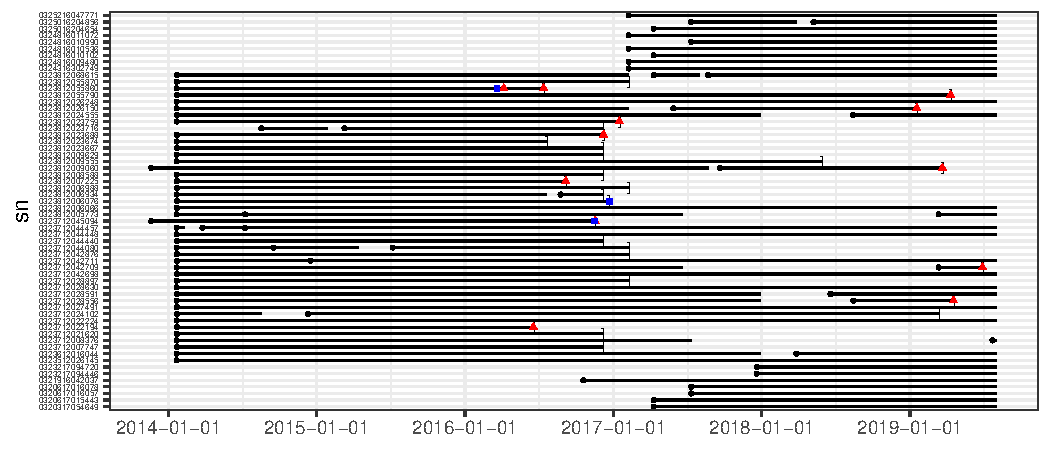
\includegraphics[width=6.5in]{figs/sample_sn.pdf}
  \caption{Serial number view of GPU life and failures. Legend: black
    dots are installs, black lines are lifetimes at installed
    location, blue squares are OTB events, red triangles are DBE
    events, and black ] are ``last seen'' events.}
  \label{fig:gpuview}
\end{figure*}
\begin{figure*}[tb]
  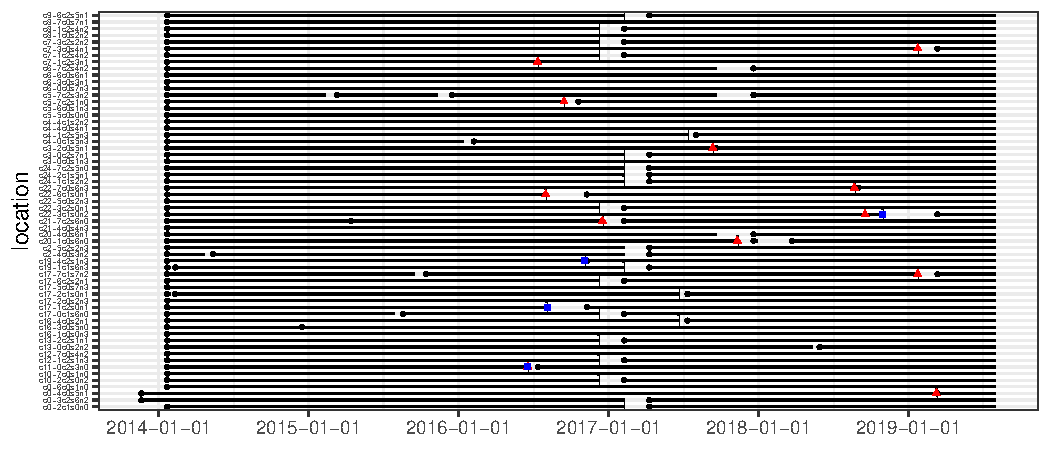
\includegraphics[width=6.5in]{figs/sample_loc.pdf}
  \caption{Location view of GPU life and failures.  Legend: black dots
    are installs, black lines are lifetimes at installed location,
    blue squares are OTB events, red triangles are DBE events, and
    black ] are ``last seen'' events.}
  \label{fig:locview}
\end{figure*}
\section{Viewing and Cleaning the Data}
\label{section:dataclean}
As we need to recover durations of GPU operation from this data, correct
processing involves time adjustments for switching between daylight
saving time and standard time and leap years. We perform this by
setting a reference time zone (Eastern time) and converting all
date-times from strings into POSIX date-time variables with the R
\pkg{lubridate} package \cite{lubridate}, which enables appropriate
date arithmetic and sensible date constructs for graphs.

As most analysis software relies on rectangular table-like data, we
fill the needed repeats of values missing in the raw data (see
Fig.~\ref{fig:dataraw}). To focus our analysis on data after the first
two rework cycles in the break-in period, we first reduce the data to
the GPUs that were installed shortly before 2014 started. This was
done by removing data for any units with a {\em remove} date before
2014. After this reduction, there were stil six older units remaining,
which we also removed to have a clean set of units for the
analysis. We do some further processing to handle time overlaps in a
tiny fraction (under 0.0007 in GPU life and 0.0002 in location life)
of recorded life in the raw records by simply dropping the overlapping
life times.

Next, we aggregate into one record per serial number with a total life
time, the first insert time, the last remove time, and a number of
other quantities such as location where the longest time is spent, the
proportion of time at the longest location, and the number of DBE or
OTB events.

To get some intuition for the GPU lifetimes on Titan, we give two
views of 60 randomly selected GPUs (Figure~\ref{fig:gpuview}) and 80
randomly selected locations (Figure~\ref{fig:locview}).
The GPU view
visually documents the life of each GPU unit: when it was installed and
removed at various locations, its DBE and OTB events, and the last
time it was seen. The location view documents the life of a location:
when different GPUs were installed and removed, their OTB and DBE
events, and whether a removal was the last time the unit was seen on
the system. These views were critical to understanding the data and to
verifying various data processing decisions.

The third rework cycle was used to label GPUs as {\em old} batch and
{\em new} batch. The two batches are clearly identifiable in the GPU
view of Fig.~\ref{fig:gpuview} as starting near 2017 timeframe. More
frequent OTB and DBE events are apparent in the old batch. It is also
clear from this view that practically all new GPUs stayed at their
initial install location whereas the old GPUs were occasionally
reinstalled at new locations. Nevertheless, a separate analysis
determined that the vast majority of time of the vast majority of
units is spent at one location by both the new and the old units.

The location view shows that each location was operational almost all
the time with small gaps when GPUs were changed out. It is also
notable that OTB and DBE events are associated with a single GPU
although four GPUs are together on a blade. The proactive replacements
in the rework cycle were done by full blades. Events on single GPUs
were usually first swapped for a new blade, the failed GPU was
replaced on the blade, and the fixed blade then reused elsewhere. The
survival analysis of Sec.~\ref{section:survival} handles these nuances
by appropriate censoring.
